\chapter{The Prediction Proccess}
\label{prediction-process}
	\section{Introduction}
		In this section, we will discuss the algorithms involved in the prediction process, a process running inside the Prediction Service, 
		and the libraries and the schematics of the predictors themselves.
	\section{Technology Stack}
		The prediction process uses several libraries to achieve its goals; the most important ones are listed below.
		\begin{itemize}
			\item Numpy linear algebra library.
			\item Scikit-learn machine learning library.
			\item torch and torchvision deep learning library.
		\end{itemize}
		\subsection{Numpy}
			\label{numpy}
			Numpy is a python compatible library, adding support for matrices and multi-dimensional arrays, along with an 
			extesive set of routines, for linear algebra operations. We use Numpy for various image transformations, spatial 
			domain image filters and dataset handling
		\subsection{Scikit-learn}
			Scikit-learn is an open-source and free machine learning library compatible with python. Includes a rich 
			ecosystem of regression and clustering algorithms, including but not limited to random forests, vector machines, 
			gradient boosting, k-means, and others. It is designed to interoperate with numerous Python numerical and scientific 
			libraries such as NumPy and SciPy.
		\subsection{pytorch and pytorchvision}
			PyTorch and pytorchvision are the python bindings of the famous torch library. Torch is a free and 
			open source deep learning and natural language processing library developed by Facebook's AI Research Lab.
	\section{Prediction Algorithms}
		In this section we will briefly discuss the two algorithms that our application currently supports, namely 
		\begin{itemize}
			\item C-Support Vector Machine, codenamed SVC v1.
			\item Residual Deep Neural Network, codenamed RESNet v18
		\end{itemize}
		\subsection{C-Support Vector Machine}
			Our first prediction algorithm, is a support vector machine[\cite{support-vector-machines}]. 
			A support vector machine is a supervised learning method that uses statistical learning frameworks[\cite{vapnik_2008}]
			to learn and classify binary datapoints, i.e., is a non-probabilistic binary linear classifier. The choice for the specific 
			classifier was based on its robustness and efficiency, especially when we have plenty of data points available. 
			\subsubsection{Prediction Process}
				The prediction process consists of 10 steps, those are.\pagebreak
				\begin{figure}[H]
					\iftrue
					\caption{SVC Prediction Process visualized}
					\centering
					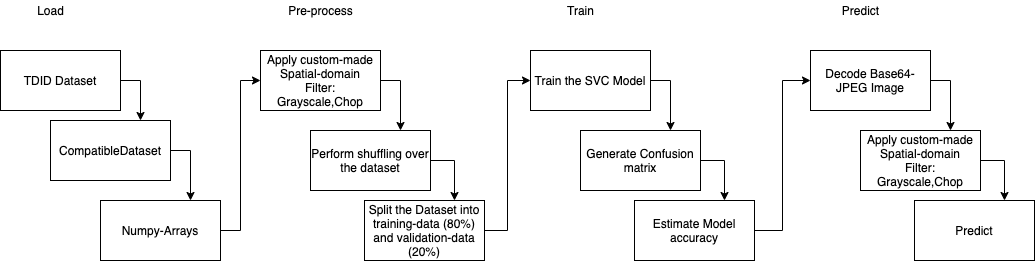
\includegraphics[angle=90,origin=c,scale=0.7]{figures/svc-process}
					\fi
				\end{figure}\pagebreak
			\subsubsection{TDID Dataset}
				TDID (Thyroid Digital Image Database) is an open database of 400 360x560  thyroid ultrasound images, as well as with XML metadata 
				about these images, such as TIRADS classification[\cite{li_ma_cui_2018}] and region of interest(region of the nodule).
				We convert the TDID Dataset images and metadata to Numpy(paragraph \ref{numpy}) arrays in the first step of the process.
			\subsubsection{Image Filters}
				After the dataset has been loaded, we apply 2 simple spatial domain filters to every ultrasound image, the filters are
				\begin{itemize}
					\item DismissRGBChannels : converts the numpy-array representation of the image to grayscale, by converting the 
					3 RGB color channels to 1 Grayscale channel.
					\item Chop : Chops the scans unessesary areas, leaving the region of interest at the center.
				\end{itemize}
			\subsection{Dataset Shuffling}
				In this step, the dataset is shuffled to ensure that the algorithm will not overfit the given data in this run.
			\subsection{Dataset-Split}
				As required in every Hold-Out 80-20 training process, in this step the dataset is splitted in training and validation data,
				in a 80\%-20\% setup.
			\subsection{Train-Validate}
				After the shuffling part is complete, the SVC Model starts training. When the training is over, we calculate the confusion matrix
				and estimate the model accuracy.
			\subsection{Predict}
				After the training is complete, our model is ready to accept the end-users ultrasound image for prediction. In this step, we
				decode the image from its original base64 and JPEG encodings, and converting it into a numpy-array(paragraph\ref{numpy}).Finally
				the SVC can predict the classification of the image.
			\subsubsection{Model Performance}
				Our model has median accuracy rate of 72\% (100000 repeats), having the following hyperparameters
				\begin{itemize}
					\item gamma=0.001
					\item C=100
				\end{itemize}
		\subsection{Residual Deep Neural Network}
			To prove the application's ability to handle deep learning models, in agreement with my supervisor, Mrs. Huizhi Liang's 
			research team, we loaded an experimental prediction model to the application to measure the application's performance. 
			The deep learning model chosen is a Residual neural network. The application handled the more complex network successfully, 
			providing the following results after 10000 runs.
			\begin{itemize}
				\item Mean Responce Time(MRT) : 3.62s
				\item Mean Memory Used : 32.7mb
				\item Mean Swap Used : 0mb
			\end{itemize}
			Those results fullfil the requirement criteria (paragraph \ref{non-functional-requirements}).
			
			
		

